\documentclass[tikz,border=10pt]{standalone}
\usepackage{tikz}
\usetikzlibrary {intersections, calc}

\begin{document}
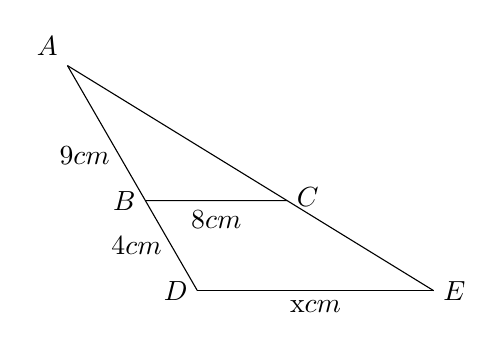
\begin{tikzpicture}[scale = 1]

%mark points on circle
        \coordinate (D) at (0,0);

        \draw (D) -- (3,0) coordinate[pos=0.5] (K) coordinate (E);
        \draw (D) -- ($(D)!1.1!120:(E)$) coordinate[pos=0.2] (P) coordinate[pos=0.4] (B) coordinate[pos=0.6] (Q) coordinate (A);
        \draw[name path = leg1] (A) -- (E);
        \node at (D) [anchor = east] {$D$};
        \node at (E) [anchor = west] {$E$};
        \node at (A) [anchor = south east] {$A$};
        \node at (B) [anchor = east] {$B$};
        
        \path[name path=leg2] (B) -- ++(0:3cm);
        \draw[name intersections={of=leg1 and leg2,by={C}}] (B) -- (C) coordinate[pos=0.5] (L);
        \node at (C) [anchor = west, yshift = 0.05cm] {$C$};

        %label lengths

        \node at (K) [anchor = north] {x$cm$};
        \node at (L) [anchor = north] {8$cm$};
        \node at (P) [anchor = east] {4$cm$};
        \node at (Q) [anchor = east] {9$cm$};
\end{tikzpicture}
\end{document}
